\section{Operational safety}
\label{sec:safety}

The ultimate goal of the assessment procedure is to determine whether a vehicle equipped with a level 4 or level 5 automation driving system (according to J3016 \cite{sae2018j3016}) is operationally safe. Therefore, before describing the assessment procedure, this section provides a brief overview of automotive safety notions and standards. 

The field of automotive safety is very broad, characterized by many types and definitions of the various aspects of safety. Nevertheless, on a high abstraction level, different types of safety are commonly distinguished, being \emph{functional safety}, \emph{cybersecurity}, \emph{safety of the intended functionality} (SOTIF). A fourth type of safety, being \emph{behavioural safety} can also be identified, relating to how the AV is programmed to behave. 

Functional safety, cybersecurity, SOTIF, and behavioural safety can be jointly referred to as \emph{operational safety}, as illustrated in \cref{fig:operational safety}. The four types of safety, as introduced here, are briefly explained in the next sections.

\begin{figure*}[b]
	\centering
	\tikzstyle{block}=[minimum width=8.5em, minimum height=4.5em, align=center, font=\small\sffamily, rounded corners=0.4em, fill=TNOlightgray]%
\begin{tikzpicture}
	%% Place the nodes
	\node[block](operational){Operational\\safety};
    \node[coordinate, below of=operational, node distance=7em](below operational){};
	\node[block, left of=below operational, node distance=5.2em](cyber){Cybersecurity};
	\node[block, left of=cyber, node distance=10.4em](functional){Functional safety\\(ISO~26262)};
	\node[block, right of=below operational, node distance=5.2em](sotif){SOTIF\\(ISO~21448)};
	\node[block, right of=sotif, node distance=10.4em](behavioural){Behavioural safety};
	
	%% Place the lines
	\node[coordinate, below of=operational, node distance=3.5em](operational helper){};
	\draw (operational) -- (operational helper) -| (functional);
	\draw (operational) -- (operational helper) -| (cyber);
	\draw (operational) -- (operational helper) -| (sotif);
	\draw (operational) -- (operational helper) -| (behavioural);
\end{tikzpicture}

	\caption{In this paper, we distinguish four aspects of operational safety: Functional safety, cybersecurity, safety of the intended functionality (SOTIF), and behavioural safety.}
	\label{fig:operational safety}
\end{figure*}



\subsection{Functional safety}
\label{sec:functional safety}

Functional safety is defined in IEC~61508 as the absence of unacceptable risk due to hazards caused by malfunctioning behaviour of systems. ISO~26262 \cite{ISO26262}, commonly referred to as ISO~26262, is an adaptation of the IEC~61508 for the automotive industry. It applies to safety-related electrical/electronic systems, specifically for road vehicles under \unit[3500]{kg}.

The ISO~26262 standard that was introduced in 2011 does not include automated vehicles. Advanced driver assistance systems (ADAS) are, however, included in the next release of ISO~26262 in 2018 \cite{ISO26262}. In ISO~26262, the notion of functional safety has been defined as follows.

\begin{definition}[Functional safety \cite{ISO26262,Dubey2017}] \label{def:functional safety}
	Functional safety is the absence of unreasonable risk due to hazards caused by malfunctioning behaviour of electrical/electronics systems.
\end{definition}

In \cref{def:functional safety}, risk refers to the combination of occurrence of harm and the severity of that harm. The malfunctioning behaviour refers to a failure or unintended behaviour of the system. According to this definition, functional safety is `looking inwards', focusing on malfunctioning AV components. 

ISO~26262 provides a guidelines from concept phase to production phase of an so-called item; that is, a system or an array of systems. This is helpful for internal safety assessment --- for development organizations --- and external safety assessment --- for independent organization. Since this work aims to provide an assessment framework for an independent assessor, it focusses especially on the start and the end of the development. This is shown in \cref{fig:ISO26262}, where an overview of ISO~26262 is presented and the focus of this work using the blue rectangles. The assessment focusses on the overall safety management, the concept phase, and the safety validation. In the remaining of this section, we will describe in more detail these parts of ISO~26262

\begin{figure*}[t]
	\centering
	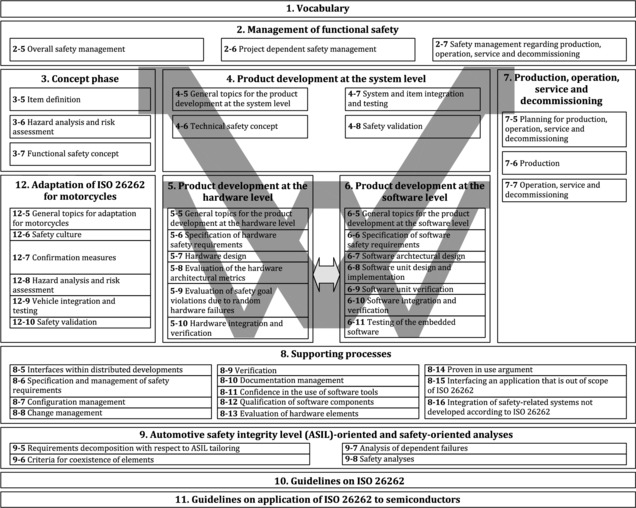
\includegraphics[width=.825\textwidth]{ISO26262_2018.png}
	\tikz[overlay]{\node[minimum height=5.2mm, minimum width=45mm, draw=TNOblue, ultra thick, rounded corners=0.4mm] at (-12.29,10.53) {};
	\node[minimum height=17.8mm, minimum width=32.5mm, draw=TNOblue, ultra thick, rounded corners=0.4mm] at (-12.95,8.8) {};
	\node[minimum height=5.7mm, minimum width=30.4mm, draw=TNOblue, ultra thick, rounded corners=0.4mm] at (-5.3,8.8) {};}
	\caption{An overview of ISO~26262. The blue rectangles denote the relevant parts for this work. The figure is based on \cite{ISO26262}.}
	\label{fig:ISO26262}
\end{figure*}

% Comment [Erwin]: Text is omitted, since it is not up to date. The safety lifecycle in the newest ISO 26262 from 2018 looks significantly different.
%The process that must be followed according to the ISO\,26262 to arrive at a functionally safe system design, the so-called `safety lifecycle', is shown in \cref{fig:ISO26262}. In the scope of AV safety assessment, the validation processes included in this lifecycle (indicated by the blue boxes in the figure) are particularly relevant; These are briefly summarized as follows.
%
%\begin{figure}[tb]
%	\centering
%	\includegraphics[width=\textwidth]{safety_lifecycle.png}
%	\tikz[overlay]{\node[minimum height=17mm, minimum width=30mm, draw=TNOblue, ultra thick, rounded corners=0.4mm] at (-0.25,8.14) {};
%		\node[minimum height=15.7mm, minimum width=31.1mm, draw=TNOblue, ultra thick, rounded corners=0.4mm] at (-0.19,4.17) {};}
%	\caption{The ISO~26262 safety lifecycle (extracted from \cite{ISO26262}).}
%	\label{fig:ISO26262}
%\end{figure}

The overall safety management of the organization developing the AV is of particular interest, because the organization and management directly impacts the functional safety of the AV \cite{yaping2019safetydriven}. In fact, the nature of safety culture is already addressed for decades in all kinds of industries \cite{choudhry2007nature}. The safety management also addresses the safety culture, which is, according to \textcite[p.~5]{piers2009safety}, defined as ``the set of enduring values and attitudes regarding safety, shared by every member of every level of an organization.'' The safety culture is typically measured through interviewing the staff. \textcite{carroll1998safety} performs a qualitative measurement of the safety culture of a departments at a nuclear power plant that reveals some issues with the safety and work culture. Therefore, such a qualitative measurement of the safety culture can positively influence the safety culture when all issues are appropriately addressed. \textcite{warszawska2016method} propose a quantitative estimation of the level of safety culture in an organization. They argue that the presented algorithm could be successfully applied in different types of the organization. \textcite{khabbazsaberi2018method} propose a method for quantitative measurement of the safety culture based on ISO~26262. Therefore, their approach might be most applicable for measuring the overall safety management of the organization developing the AV.

According to ISO~26262, the concept phase consists of three steps: the item definition, the hazard analysis and risk assessment (HARA), and the functional safety concept. Whereas the item can refer to a function of the vehicle, in our case it is referring to the AV as a whole. The objective of the item definition is ``to define and describe the item, its dependencies on, and interaction with, the environment and other items; and to support an adequate understanding of the item so that the activities in subsequent phases can be performed'' \cite[Clause 3.5]{ISO26262}. A crucial element of the item definition is the definition of the operating conditions since the AV is unlikely to operate under all conditions \cite{koopman2016challenges}. The item definition is an important input for the assessment and, therefore, the vehicle, the ODD, and the DDT need to be defined when applying for the assessment.

The objective of the HARA is ``to identify and to categorise the hazardous events caused by malfunctioning behaviour of the item; and to formulate the safety goals related to the prevention or mitigation of the hazardous events, in order to avoid unreasonable risk'' \cite[Clause 3.6]{ISO26262}. Using a HARA to assess the risks is already done for decades \cite{sage1980methodologies}. \textcite{johansson2015importance} discusses the use of a HARA for AVs and, especially, the completeness of the HARA. \textcite{johansson2015importance} further argues that elaborating the HARA --- instead of defining only few general safety goals --- results in a potential to significantly save costs because of the large implications of general safety goals on the whole AV. For an example of an HARA for an AV, see \cite{stolte2017hara}. As part of the HARA, the hazards are categorised according to the Automotive Safety Integrity Level (ASIL). The ASIL is based on qualitative scores for the severity (the estimate of the extent of harm), the controllability (the ability to avoid a specified harm or damage), and the probability of exposure (the state of being in an operational situation). The ASIL determines to what extent certain measures need to be taken to minimize a risk. Since the ASIL is based on qualitative experts' judgements, it is not always reliable \cite{khastgir2017towards}. As such, several attempts are made to make the HARA more objective; for example using a rule-set for determining the scores of the severity, controllability, and exposure \cite{khastgir2017towards}. \textcite{duracz2015rigorous} use simulations to support the HARA. Another possibility is to use real-life driving data and simulations to arrive to a quantitative measure for risk \cite{degelder2019risk}.

The functional safety concept \cite[Clause 3.8]{ISO26262} involves specification of functions and their interactions which are necessary to achieve the desired safe behaviour as defined by the safety goals resulting from the HARA. 

\todo{Check whether the functional safety concept should be part of this report. Do we assess the functional safety concept? I (Erwin) cannot see it immediately in the document review.}

The safety validation checks, on a vehicle level, whether the safety goals are fulfilled. This is done through virtual and physical testing, representing the `intended use cases', i.e., the traffic scenarios as they occur in the envisioned operational environment of the AV.

\begin{remark}
	Intuitively, one might think that (safety) \emph{verification} is more appropriate to indicate the main assessment objective. ISO\,26262, however, defines verification as ``determination of completeness and correct specification, or implementation, of requirements from a phase or sub-phase,'' which clearly makes this notion less suitable to express the assessment objective.
\end{remark}

%When adopting the selected topics of the lifecycle, a first step is made towards a process for safety assessment of AVs from the perspective of functional safety; This is visualized in \cref{fig:functional safety assessment}, where the scenario generation component, which is not explicitly included in the original ISO process, aims to generate relevant traffic scenarios (either or not as part of overarching `use cases').
%
% Erwin: I removed figure, because I do not see the added value (anymore)
%\begin{figure}[tb]
%	\centering
%	\includegraphics[scale=1]{functional_safety_assessment.pdf}
%	\caption{Functional safety assessment steps, inspired by the ISO~26262.}
%	\label{fig:functional safety assessment}
%\end{figure}

%From the information presented in this section, it can be concluded that the ISO~26262 standard is oriented towards development of a certain automation functionality, as part of which verification and validation processes are implemented. The objective of the assessment pipeline, however, is not to design a safe AV but to assess the safety of a given design. Consequently, the process from \cref{fig:functional safety assessment} needs to be further adapted, both in terminology and in contents, to better fit this objective. The next chapter (in particular \cref{sec:document review}) will further specify the role of the safety validation process in the assessment procedure, as a start for further development of the pipeline.


\subsection{Cybersecurity}
\label{sec:cybersecurity}

Whereas functional safety focusses on hazards caused by malfunctioning behaviour of components \emph{inside} the vehicle, cybersecurity focusses on threats from \emph{outside} the vehicle. Cybersecurity is a broadly used term and many different definitions exist; see \cite{craigen2014defining} for an overview of existing definitions. TR68-3 \cite[p.~9]{tr68cybersecurity} defines cybersecurity as ``the protection of electronic systems from cyberattacks'', where a cyberattack is defined as ``an assault on an electronic system to violate its confidentiality, integrity, or availability through cybersecurity means [...]'' \cite[p.~9]{tr68cybersecurity}. \textcite[p.~1]{lewis2006cybersecurity} writes that ``cybersecurity entails the safeguarding of computer networks and the information they contain from penetration and from malicious damage or disruption.'' Throughout this work, we adopt the definition from \textcite{craigen2014defining}, which resulted from an in-depth literature review and multiple discussions on cybersecurity with practitioners, academics, and graduate students:

\begin{definition}[Cybersecurity \cite{craigen2014defining}]
	Cybersecurity is the organization and collection of resources, processes, and structures used to protect cyberspace and cyberspace-enabled systems from occurrences that misalign \textup{de jure} from \textup{de facto} property rights.
\end{definition}

AVs will be increasingly connected; for example using vehicle-to-vehicle and vehicle-to-infrastructure communications and Internet of Things devices connected to the vehicle, such as bluetooth-connected mobile phones. With respect to cyber attacks, a connected device means an exposed device. As such, an autonomous vehicle is a highly exposed device that relies heavily on its hackable software. Cybersecurity needs to be considered as the cyber attacks may lead to major safety losses \cite{hashemeiza2017sharks}.

Because of the many connections an AV has with its outside world, there are many cyber threats. The driving behaviour can be controlled by attacked the internal bus system of an AV \cite{wolf2004security}, possibly through the on-board diagnostics port that every modern car has \cite{checkoway2011comprehensive}. Vehicle-to-vehicle communications using dedicated short range communications are exposed to, amongst others, denial-of-service attacks \cite{lyamin2014real} and false messages \cite{moalla2012risk}. Since the AV depends on its software, it is vulnerable to malware attacks \cite{zhang2014defending}. Connected a vehicle to a mobile device introduce other security challenges \cite{yan2015twoyear, oka2014bluetooth}. Because an AV heavily relies on its sensors, it is also exposed to spoofing attacks \cite{yan2016can, davidson2016controlling}, which utilizes the underlying principles of sensors to blind or deceive them. For an overview of different cyber threats, see \cite{cui2018review, hashemeiza2017sharks, studnia2013survey, yaugdereli2015study, vanderheijden2016survey, sakiz2017survey, zheng2016investigating}. 

TR68-3 \cite[p.~12]{tr68cybersecurity} lists four key cybersecurity principles, ``referenced and in-line with industry best practices'', which are security by design, defence in depth, continuous operational management and oversight, and resiliency. Security by design \cite{ross2018systems, chattopadhyay2018autonomous} means that the cybersecurity implementation is considered from the start of the design of the product, rather than addressing specific attacks in an isolated and ad-hoc manner. This also includes formal validation and verification steps prior to the release of the product. Defence in depth, also referred to as Castle Model \cite{leuprecht2016beyond}, requires a holistic approach to cybersecurity built into all layers of the system architecture to ensure integrated and comprehensive protection of the entire system. Continuous operational management and oversight includes the prediction of potential threats \cite{gandotra2015computational}, the detection of attacks, and effective responds to attacks. Whereas cybersecurity mostly focusses on known attacks, cyber resilience is about ensuring that the system is prepared for the event of an unforeseeable and unpredictable attack \cite{sharkov2016cybersecurity}.

%\begin{itemize}
%	\item \emph{Security-by-design}: This means that the cybersecurity implementation needs to be systematic and process-oriented. Furthermore, it includes formal validation and verification steps prior to product release.
%	\item \emph{Defence-in-depth}: This requires a holistic approach to cybersecurity built into the system architecture to ensure integrated and comprehensive protection of the entire system.
%	\item \emph{Continuous operational management and oversight}: The cybersecurity operations need to be continuously operational and include predicting potential threats, detecting attacks, and responding effectively.
%	\item \emph{Resiliency}: Resiliency is about ensuring that cybersecurity preparedness and readiness is in place ready for the event of an incident.
%\end{itemize}

\subsection{Safety of the intended functionality}
\label{sec:sotif}

\todo{Link section with TR68-2. Provide more references.}

As mentioned earlier, functional safety is `inward looking', in the sense that it focuses on malfunctioning AV components, which include the vehicle platform, sensors and automation system. For AVs, however, it is also important to `look outwards', i.e., to include inherent sensor and perception system limitations in the safety assessment framework and to take decision-making capabilities of the AV into account. These aspects of AV safety are covered by the notion of \emph{safety of the intended functionality} (SOTIF).

SOTIF relates to hazardous behaviour which is not caused by a malfunction. In particular for AVs, SOTIF is often related to environmental perception \cite{Fischer2017} since environmental sensors typically have inherent limitations, which may cause the AV to behave unsafely. Examples of such limitations are the occurrence of so-called `ghosts' in radar measurements, or the blinding effect of direct sunlight in case of camera systems. It is important to mention that SOTIF is assessed on a system level, as opposed to functional safety, which is focusing on the AV component level. This type of safety is described in the standard ISO/WD\,PAS\,21448, in short referred to as ISO\,21448, which is currently under development \cite{ISO21448}. This draft standard defines SOTIF in a very broad sense as ``the absence of unreasonable risk of the intended functions''. In the scope of the current document, a more precise definition will be adopted, as proposed below. 

\begin{definition}[Safety of the intended functionality]
	Safety of the intended functionality (SOTIF) is the ability of the automation system to correctly comprehend the environmental situation and behave safely, by ensuring that the AV systems and components are operating within their design boundaries and, if they are not, by activating appropriate countermeasures.
\end{definition}

\subsection{Behavioural safety}
\label{sec:behavioural safety}

\todo{Link section with TR68-1. Provide more references.}

Whereas ISO\,21448 intends to facilitate safe functionality and ultimately provide sufficiently detailed and robust object and event detections, there is another type of safety that involves using these detections to correctly interpret the traffic situation and subsequently safely discharge manoeuvre planning. This can be captured by the notion of \emph{behavioural safety}, which, in a recent report by Waymo \cite{Waymo2017}, is introduced as ``An aspect of system safety that focuses on how a system should behave normally in its environment to avoid hazards and reduce the risk of mishaps: for instance, detect objects and respond in a safe way (slow down, stop, turn, lane change, etc.).'' This type of safety thus addresses the AV behaviour as intentionally programmed by the developer, with all components and systems of the AV operating as intended. A relevant question in this context is, for instance, whether the AV follows the traffic rules. Since it is questionable whether this type of safety will be part of the final version of ISO\,21448, behavioural safety is regarded as a third type of safety.

The UN-ECE Automatically Commanded Steering Function group is drafting amendments to UN-ECE Regulation 79 which describes the expected behaviour of a level 3 automated driving system \cite{sae2018j3016}. However, the scope is limited to well-structured and controlled highways where there are no pedestrians/bicycles, at least two lanes in the direction of travel, and a physical separation between contraflow traffic. The authors are not aware of existing art describing the behavioural safety requirements for a level 4 automated driving system operating in complex urban environments, hence this study aims to provide some definition to the behavioural characteristics required for a vehicle using the context of Singapore's road traffic rules and traffic environment as the case study. The proposed assessment methodology makes use of traffic scenarios to assess the behavioural safety of the AV. The safety assessment procedure, which is described in \cref{sec:assessment}, sets out how the scenarios are defined from a Document review exercise and from scenario generation using acquisition of real-world driving data. Next, the AV's behavioural performance is assessed through virtual and physical safety validation using these scenarios.
